\chapter{Introducción}
\label{cap:capitulo1}
\setcounter{page}{1}

Este capítulo sitúa TierraViva dentro del contexto de la digitalización agrícola y del riego inteligente. A partir de una necesidad práctica (supervisar y actuar sobre el riego sin depender siempre de una revisión presencial) se introduce el problema técnico, la motivación del trabajo, su alcance y la organización de la memoria.

\section{Contexto general: agricultura, agua y digitalización}
\label{sec:contexto_general}

La agricultura es una de las actividades en las que el uso eficiente de los recursos tiene un impacto más directo, tanto desde el punto de vista económico como medioambiental. Entre todos los recursos implicados, el agua ocupa un papel especialmente importante, ya que condiciona de forma directa el desarrollo de los cultivos y, al mismo tiempo, es un recurso limitado que debe gestionarse con cuidado. Según AQUASTAT, base de datos internacional sobre agua y agricultura, el uso agrícola supone alrededor del 69\% de las extracciones mundiales de agua \cite{fao_aquastat_water_use}. En este contexto, el riego no puede entenderse únicamente como una tarea rutinaria, sino como una decisión técnica que depende de múltiples factores: el estado del suelo, las condiciones ambientales, el tipo de cultivo, la época del año y la disponibilidad de agua.

Tradicionalmente, muchos sistemas de riego se han basado en criterios fijos, como horarios predefinidos o estimaciones manuales del estado del terreno. Aunque este enfoque puede ser suficiente en determinadas situaciones, existen limitaciones claras. Un riego programado de forma rígida puede aportar agua cuando no es necesario o, por el contrario, no hacerlo en momentos en los que el cultivo sí lo necesita. Esta falta de adaptación al estado real del entorno puede traducirse en un consumo innecesario de agua, un peor aprovechamiento de los recursos y una menor capacidad de respuesta ante cambios de temperatura, humedad o exposición solar.

\begin{figure}[H]
    \centering
    \makebox[\textwidth][c]{%
        
\includegraphics[width=1.15\textwidth]{figs_png/riegoTrad_riegoInt.png}%
    }
    \caption{Evolución conceptual desde un riego basado en rutinas fijas hacia un riego apoyado en medidas reales del entorno. Elaboración propia.}
    \label{fig:cap1_rutina_a_criterio}
\end{figure}

Para dar solución a estas limitaciones, la digitalización del entorno agrícola proporciona las herramientas necesarias para desarrollar sistemas informados y adaptativos. Mediante el despliegue de redes de sensores y equipos de comunicación, es posible adquirir datos en tiempo real y observar el estado del entorno de forma continua. Este planteamiento se relaciona directamente con la agricultura de precisión, cuyo objetivo no es únicamente automatizar tareas, sino utilizar información del propio entorno para mejorar la eficiencia, reducir desperdicios y facilitar la gestión de los recursos.

En este tipo de sistemas, la monitorización ambiental desempeña un papel fundamental. Medir variables como la humedad del suelo, la temperatura, la humedad relativa, la presión atmosférica o la luminosidad permite disponer de una visión más completa del estado de una zona de cultivo, y no todas estas variables tienen el mismo peso en la decisión de riego. Por ejemplo, la humedad del suelo puede indicar de forma directa la necesidad de aportar agua, mientras que la temperatura o la luz ambiental ayudan a interpretar las condiciones en las que se está produciendo la evaporación o el déficit de agua.

La automatización del riego aparece, por tanto, como una evolución natural de la monitorización. Un sistema que únicamente muestra datos puede ser útil para el agricultor, pero sigue dependiendo de una intervención manual para actuar. En cambio, un sistema capaz de medir, analizar y accionar un elemento de riego permite cerrar el ciclo completo: observar el entorno, interpretar su estado y ejecutar una acción cuando se cumplen determinadas condiciones. Esta capacidad resulta especialmente interesante en zonas donde la supervisión constante no siempre es posible o donde se quiere reducir la dependencia de decisiones manuales repetitivas.

Además, en muchos escenarios agrícolas o rurales existen limitaciones de infraestructura que condicionan el diseño de cualquier solución tecnológica. No siempre se dispone de una red WiFi (\textit{Wireless Fidelity}) estable, alimentación eléctrica cercana o cobertura de red garantizada. Por ello, un sistema de riego inteligente no debe plantearse únicamente desde el punto de vista del software o de la sensorización, sino como una integración completa de hardware, comunicaciones, energía, almacenamiento de datos y actuación física sobre el riego. La dificultad real no está solo en medir una variable, sino en conseguir que todos estos elementos funcionen de forma coordinada y fiable.

\begin{wrapfigure}{r}{0.32\textwidth}
    \vspace{-12pt}
    \centering
    
\includegraphics[width=0.30\textwidth]{figs/TierraViva_LogoFinal.jpeg}
    \caption{Identidad visual de TierraViva.}
    \label{fig:logo_tierraviva}
    \vspace{-8pt}
\end{wrapfigure}

Dentro de este contexto surge TierraViva, un proyecto orientado al diseño de un prototipo de Internet de las Cosas (IoT, del inglés \textit{Internet of Things}) para monitorización y control de riego. El objetivo principal no es construir un producto agrícola industrial cerrado, sino desarrollar una solución funcional que permita comprobar cómo diferentes tecnologías pueden integrarse para resolver un problema real. El proyecto parte de una idea sencilla, medir el estado del entorno y actuar sobre el riego cuando sea necesario, pero implica varias capas técnicas: adquisición de datos mediante sensores, comunicación remota, publicación de telemetría, almacenamiento, visualización, lógica local de decisión en las estaciones y actuación física sobre el sistema de riego.

Por tanto, este trabajo se sitúa en la intersección de varias disciplinas: agricultura de precisión, IoT, comunicaciones y sistemas embebidos. Esta combinación permite abordar un problema práctico desde una perspectiva propia de la ingeniería: analizar necesidades, estudiar alternativas, justificar decisiones, implementar un prototipo y validar su funcionamiento mediante pruebas. La finalidad última es demostrar que una arquitectura bien diseñada puede ayudar a mejorar la gestión del riego, aportando información objetiva y capacidad de actuación automática o supervisada.

\section{Motivación del proyecto}
\label{sec:motivacion_origen}

La motivación de este proyecto surge de la dificultad de gestionar correctamente el riego en pequeños cultivos o huertos que no pueden supervisarse de forma continua. En estos escenarios, especialmente en épocas de más calor, pueden aparecer problemas tanto por falta de agua como por exceso de riego. Aunque pueda parecer una situación sencilla, refleja una necesidad habitual: cuidar correctamente un terreno cuando no se está físicamente allí de forma continua.

Detrás de esa necesidad existe un problema técnico real. No se trata solo de regar más o menos, sino de saber cuándo hace falta regar, en qué condiciones se encuentra el terreno y si sería posible actuar sin depender siempre de una revisión manual. Por tanto, el interés del proyecto no está únicamente en automatizar una tarea, sino en diseñar un sistema capaz de observar el entorno, interpretar su estado y actuar de forma controlada.

La idea inicial puede entenderse como una solución de aviso remoto, pero al analizar el caso con más detalle aparecen cuestiones que hacen el problema más interesante: la cobertura en entornos rurales, la alimentación del sistema, la necesidad de funcionamiento desatendido, la fiabilidad de las comunicaciones y la posibilidad de controlar físicamente el riego.

La evolución natural de esta idea conduce hacia un sistema más completo de monitorización y control. El proyecto no consiste únicamente en conectar sensores, sino en diseñar una arquitectura capaz de integrar distintas áreas de la ingeniería de forma coherente. Esta integración es una de las partes más relevantes del trabajo, porque permite transformar una necesidad cotidiana en un problema técnico con suficiente profundidad para un Trabajo Fin de Grado (TFG).

Otro aspecto importante en la motivación es que TierraViva permite aplicar conocimientos que normalmente se estudian por separado. En el proyecto intervienen electrónica, programación embebida, comunicaciones, bases de datos, desarrollo web, visualización de información y control de actuadores. Esta combinación hace que el trabajo sea más exigente, pero también más representativo de un sistema real, donde el valor no está solo en que cada parte funcione de manera aislada, sino en conseguir que todas trabajen coordinadamente.

Además, el proyecto tiene una componente práctica y sostenible que lo hace especialmente atractivo. El objetivo no es desarrollar tecnología por sí misma, sino utilizarla para responder a una necesidad concreta: gestionar mejor el riego y reducir decisiones basadas únicamente en intuición, costumbre u horarios fijos. En este sentido, TierraViva conecta la ingeniería con una aplicación tangible, cercana y fácil de entender, pero con suficiente profundidad técnica como para justificar un desarrollo completo.

Desde esta perspectiva, el proyecto se relaciona con varios Objetivos de Desarrollo Sostenible, especialmente con el ODS 2, vinculado a prácticas agrícolas más sostenibles; el ODS 6, relacionado con un uso más eficiente del agua; el ODS 12, asociado a una gestión responsable de recursos; y el ODS 13, orientado a mejorar la capacidad de adaptación ante condiciones ambientales variables \cite{onu_ods2,onu_ods6,onu_ods12,onu_ods13}.

Esta relación debe interpretarse dentro del alcance real del TFG: TierraViva no demuestra todavía una mejora agronómica prolongada ni cuantifica ahorro hídrico, pero desarrolla una arquitectura técnica capaz de medir, registrar, actuar de forma controlada y sentar las bases para futuras validaciones de impacto ambiental y social. La valoración final de esta alineación se retoma en el Capítulo~\ref{cap:resultados_discusion_conclusiones}.

\section{Planteamiento del problema}
\label{sec:planteamiento_problema}

El reto principal de este TFG es transformar una situación tradicionalmente manual en un sistema monitorizado, trazable y parcialmente automatizado.

El primer aspecto del problema es la \textbf{adquisición de datos}. Para que el sistema pueda tomar decisiones con cierto criterio, necesita disponer de medidas representativas del entorno. La humedad del suelo es la variable más directamente relacionada con la necesidad de riego, pero no es la única información útil, ya que otras variables como la temperatura, la humedad relativa o la luminosidad permiten contextualizar mejor el estado de la zona monitorizada. El sistema debe ser capaz de leer estas magnitudes de forma periódica y convertirlas en datos utilizables, evitando que las lecturas queden como valores aislados sin relación con el funcionamiento global del sistema.

El segundo aspecto es la \textbf{transmisión de la información}. En un sistema de riego desatendido, las estaciones de campo no pueden depender de una supervisión constante ni de una conexión física permanente a un ordenador. Los datos deben poder enviarse desde la zona donde se encuentran los sensores hasta un punto donde puedan ser procesados, almacenados y visualizados. Esta comunicación debe ser suficientemente fiable para que el agricultor o el usuario pueda conocer el estado del sistema, pero también debe tener en cuenta las limitaciones propias de un entorno rural, donde no siempre existe una infraestructura de red estable.

Una vez recibidos los datos, el siguiente problema es su \textbf{almacenamiento y tratamiento}. Mostrar una lectura puntual puede servir para una comprobación rápida, pero no permite analizar la evolución del sistema. Para que el prototipo tenga utilidad real, es necesario registrar las medidas recibidas, asociarlas a una estación concreta y conservar un histórico. De esta forma, se puede comprobar cómo varían las condiciones del entorno a lo largo del tiempo, detectar comportamientos anómalos y justificar las decisiones de riego tomadas por el sistema.

La \textbf{visualización} también forma parte del problema. Un sistema técnico puede estar funcionando correctamente de manera interna, pero si el agricultor o el usuario no puede interpretar su estado de forma clara, su utilidad queda limitada. Por ello, es necesario disponer de una interfaz que permita consultar las últimas lecturas, observar la evolución de las variables principales y conocer el estado del riego. Esta interfaz debe presentar la información de forma comprensible, sin exigir que el usuario tenga que interpretar directamente datos brutos, mensajes de consola o registros internos difíciles de entender para alguien no experto.

Otro punto fundamental es la \textbf{toma de decisiones}. El sistema debe ser capaz de determinar cuándo conviene actuar sobre el riego a partir de las medidas disponibles. En el alcance de este TFG, esta decisión se plantea mediante reglas verificables, como umbrales, condiciones de seguridad y tiempos máximos de actuación. Este enfoque resulta adecuado para un prototipo, ya que permite justificar de forma clara por qué se activa o se detiene el riego, sin depender de modelos predictivos complejos que requerirían una cantidad elevada de datos históricos para entrenarse y validarse correctamente.

El último elemento del problema es la \textbf{actuación física}. Un sistema que solo mide y muestra información se queda en una solución de monitorización. Para avanzar hacia un sistema de riego inteligente, es necesario cerrar el ciclo mediante el control de un actuador. Esto introduce requisitos adicionales de seguridad, ya que una lectura incorrecta, una regla mal configurada, una pérdida de comunicación o un fallo eléctrico no deben provocar que la bomba permanezca activa indefinidamente. Por tanto, el diseño debe contemplar un comportamiento seguro por defecto dentro de la propia estación de campo, priorizando la desactivación de la bomba ante situaciones de error.

En conjunto, el problema planteado puede entenderse como un problema de integración de subsistemas. TierraViva debe coordinar sensores, estación de campo, comunicación remota, plataforma de publicación de datos, sistema de supervisión, interfaz de usuario y actuador. Cada una de estas partes tiene una función concreta, pero el valor del proyecto aparece cuando todas trabajan de forma conjunta. Por esta razón, el desarrollo no se limita a seleccionar componentes, sino que exige definir una arquitectura modular, validar cada bloque por separado y comprobar posteriormente el funcionamiento del sistema completo.

Además, el sistema se diseña pensando en su posible ampliación. Aunque el prototipo pueda validarse inicialmente con una estación, la arquitectura permite incorporar nuevas estaciones de campo, nuevas variables medidas o nuevos mecanismos de decisión. Esta modularidad es importante para que el trabajo no quede como una solución cerrada y difícil de extender, sino como una base sobre la que puedan plantearse mejoras futuras, como autonomía energética, despliegue multizona o mecanismos predictivos basados en datos históricos.

\section{Alcance y limitaciones}
\label{sec:alcance_limitaciones}

El objetivo no es desarrollar un producto comercial cerrado ni una solución industrial certificada, sino construir una arquitectura completa que permita comprobar, de forma experimental, cómo diferentes tecnologías pueden integrarse para resolver un problema real. Por tanto, el trabajo se evalúa principalmente desde el punto de vista de la integración tecnológica, el funcionamiento del sistema y la validación mediante pruebas.

El prototipo debe ser capaz de medir variables relevantes del entorno, transmitir la información obtenida, registrar o consultar los datos recibidos, permitir su visualización y actuar sobre el riego bajo determinadas condiciones evaluadas localmente en cada estación. De esta forma, el proyecto no se limita a una prueba aislada de sensores ni a una aplicación de visualización, sino que busca cerrar el ciclo completo de monitorización, decisión y actuación. Esta integración constituye el núcleo del trabajo y permite valorar el sistema como una solución IoT aplicada a un caso práctico.

\begin{figure}[htbp]
    \centering
    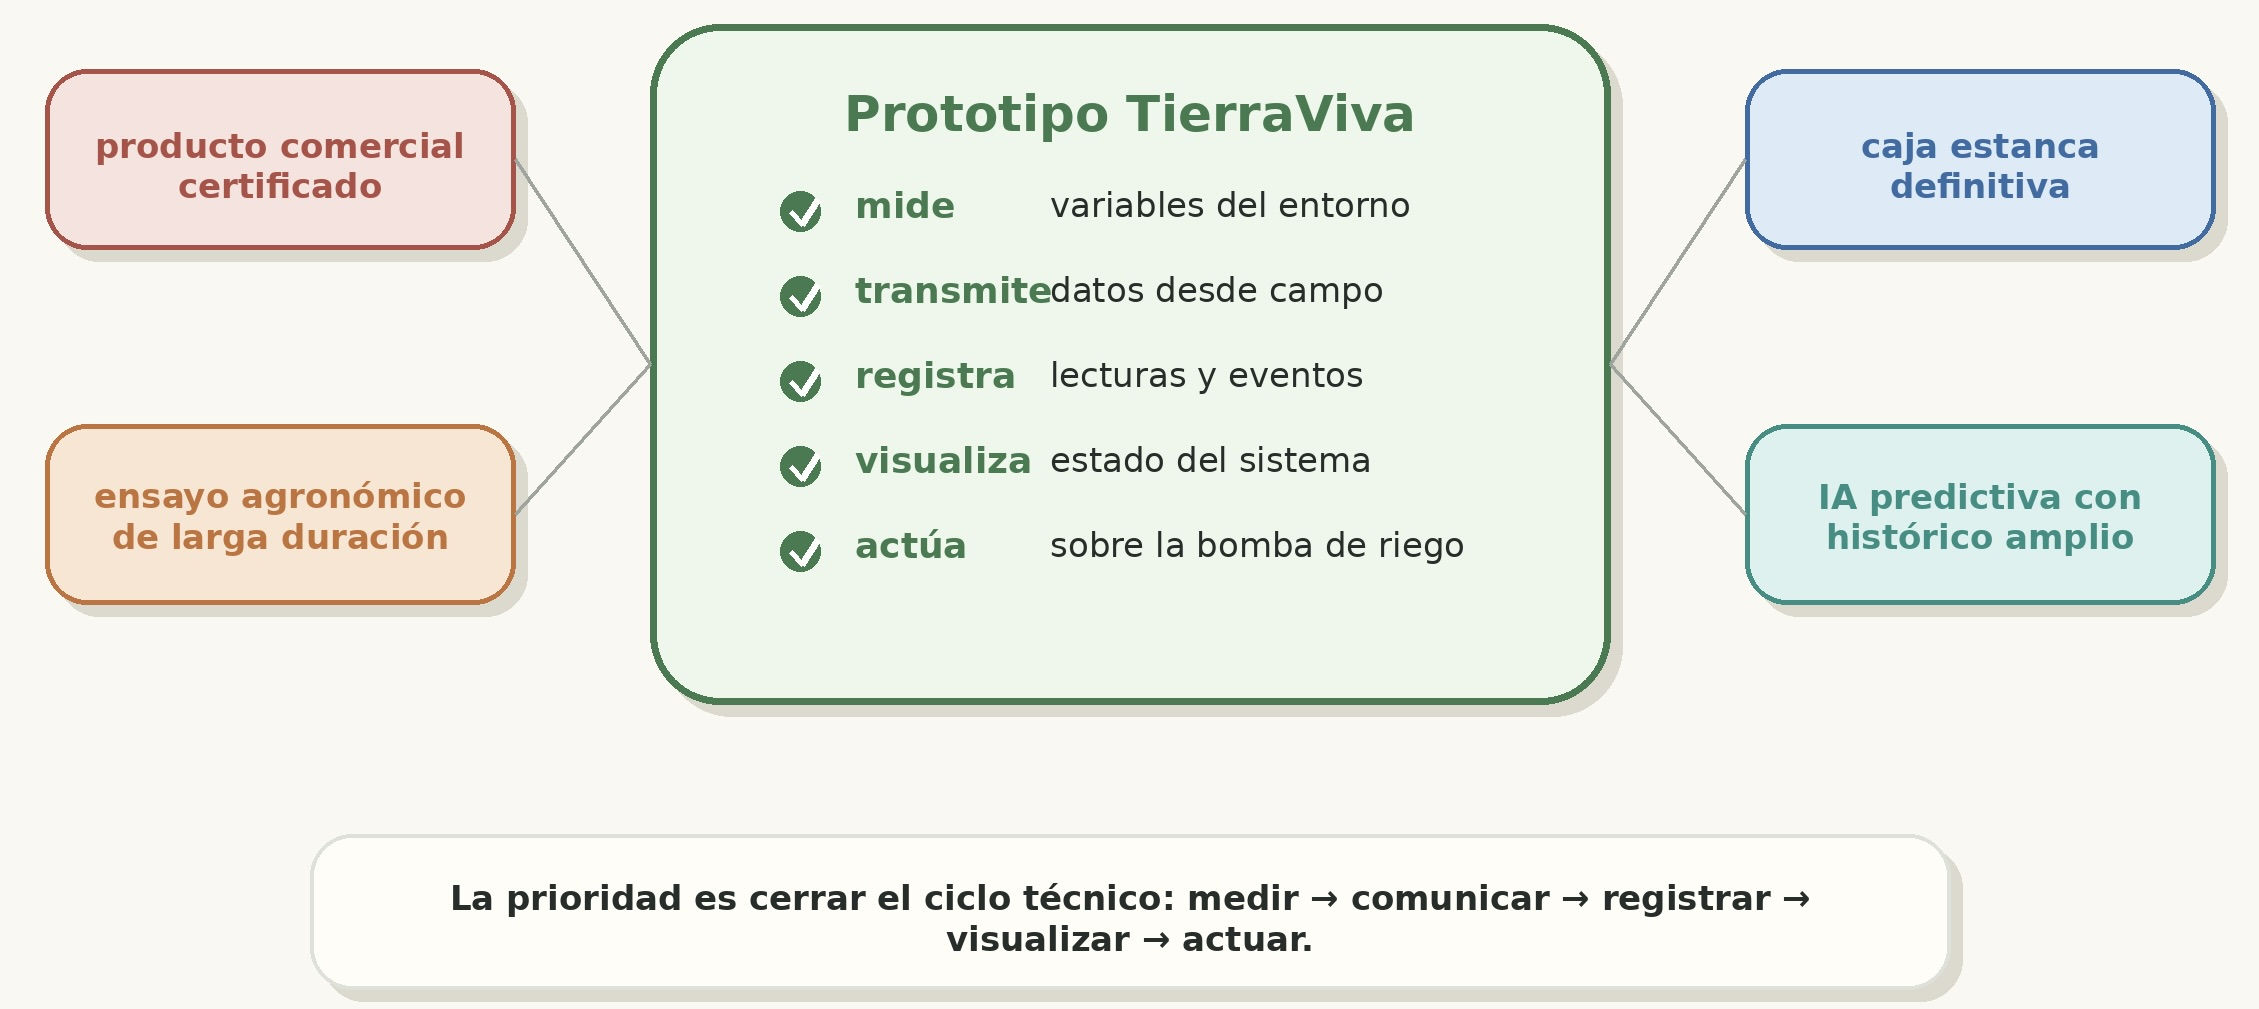
\includegraphics[width=0.96\textwidth]{figs/fig_cap1_05_alcance_prototipo.jpeg}
    \caption{Delimitación del alcance del prototipo TierraViva y de los aspectos que quedan fuera de esta fase del trabajo. Elaboración propia.}
    \label{fig:cap1_alcance_prototipo}
\end{figure}

No obstante, es importante delimitar claramente el alcance para evitar interpretar el proyecto como un sistema agrícola final preparado para su instalación directa en cualquier explotación. El prototipo desarrollado no pretende sustituir a soluciones profesionales de riego industrial, ni contempla certificaciones eléctricas, hidráulicas o de comunicaciones. Tampoco se aborda el diseño mecánico definitivo de una caja estanca, la fabricación de una placa electrónica propia ni la optimización completa del consumo energético para funcionamiento durante largos periodos sin mantenimiento.

Otra limitación relevante es la validación agronómica. Aunque el sistema está orientado al riego y se basa en variables relacionadas con el estado del entorno, no se realizará un ensayo prolongado durante varios meses sobre un cultivo real. Una validación de ese tipo requeriría controlar factores externos como el tipo de suelo, la especie cultivada, la climatología, la frecuencia de riego, la evolución del crecimiento de las plantas y la comparación con métodos tradicionales. En este TFG, la validación se centrará en comprobar que el prototipo mide, comunica, registra, visualiza y actúa correctamente, dejando los ensayos agronómicos de larga duración como una posible línea futura.

También se establece como limitación el uso de inteligencia artificial. Aunque el proyecto se plantea dentro de un contexto en el que la analítica de datos y los mecanismos predictivos pueden aportar mucho valor, no tendría rigor presentar como inteligencia artificial una lógica basada únicamente en reglas o umbrales. Para implementar modelos predictivos fiables sería necesario disponer de un histórico amplio de datos, recogido durante suficiente tiempo y bajo condiciones representativas. Por ello, en este trabajo la toma de decisiones se planteará de forma verificable mediante reglas, dejando la inteligencia artificial como una ampliación futura si se dispone de datos suficientes para entrenar, validar y justificar un modelo.

El sistema se diseñará con una visión modular, de modo que pueda ampliarse posteriormente con nuevas estaciones, nuevas variables medidas, mejoras en la autonomía energética o mecanismos más avanzados de análisis. Sin embargo, dentro del alcance de esta memoria, la prioridad será demostrar que la arquitectura propuesta funciona de extremo a extremo: desde la adquisición de datos en campo hasta la visualización y actuación sobre el riego. Esta delimitación permite mantener un equilibrio entre ambición y viabilidad, evitando prometer funcionalidades que no puedan ser implementadas y validadas con suficiente solidez durante el desarrollo del TFG.

Asimismo, en los capítulos finales de la memoria se incorporará una valoración del impacto social y ambiental del proyecto. Esta valoración analizará de qué forma TierraViva contribuye potencialmente a las metas ODS identificadas, especialmente en relación con agricultura sostenible, eficiencia en el uso del agua y gestión responsable de recursos. También se señalarán las limitaciones que impiden afirmar todavía un impacto cuantificado, así como posibles aspectos pendientes de mejora, como la optimización energética, la durabilidad del prototipo o la validación agronómica prolongada.

En resumen, el alcance del proyecto es el de un prototipo funcional, documentado y validado, orientado a demostrar la viabilidad técnica de un sistema IoT para riego inteligente. Sus limitaciones no se consideran una debilidad del trabajo, sino una forma de definir con precisión qué se ha implementado, qué se ha probado y qué queda abierto para futuras fases de desarrollo.

\section{Organización de la memoria}
\label{sec:organizacion_memoria}

La memoria se organiza de forma progresiva, comenzando por la introducción del problema y avanzando después hacia los fundamentos técnicos, las decisiones de diseño, la implementación y la validación del sistema.

En el Capítulo 1 se presenta el contexto del proyecto, la motivación, el planteamiento del problema y el alcance del trabajo. El Capítulo 2 recoge el estado del arte y los fundamentos tecnológicos necesarios para comprender la solución propuesta, incluyendo arquitecturas IoT, agricultura de precisión, comunicaciones, plataformas cloud y automatización del riego.

El Capítulo 3 describe los métodos, materiales y decisiones de diseño, definiendo los requisitos del sistema, la metodología seguida, la arquitectura general planteada y la justificación de las principales elecciones tecnológicas. A continuación, el Capítulo 4 presenta la arquitectura final de TierraViva y explica cómo se integran las estaciones de campo, la plataforma cloud, la Raspberry Pi como sistema de supervisión y los mecanismos locales de actuación.

Los Capítulos 5 y 6 se centran en la implementación del prototipo. El primero aborda la parte \textit{hardware} y \textit{firmware} de las estaciones, incluyendo la lectura de sensores, la publicación de telemetría y la decisión local de riego, mientras que el segundo describe la implementación software de supervisión en Raspberry Pi y nube. Posteriormente, el Capítulo 7 recoge la validación y las pruebas realizadas, desde la comprobación por bloques hasta la prueba funcional en Agrolab Móstoles.

Finalmente, el Capítulo 8 integra los resultados obtenidos, la discusión técnica de la solución, la valoración cualitativa recibida durante la prueba en Agrolab, las limitaciones detectadas, las líneas de trabajo futuro y las conclusiones finales del Trabajo de Fin de Grado.